\section{Implementation}
%%%%%%%%%%%% MID WAY AGENDA %%%%%%%%%%%%%%
%\begin{frame}<beamer>
%\frametitle{Thomas Holm Pilgaard}
%\tableofcontents[currentsection]
%\end{frame}
%%%%%%%%%%%% MID WAY AGENDA %%%%%%%%%%%%%%

\begin{frame}{Parameter identification results}{Wrong measurement data}

\begin{itemize}
	 	\item<1-> Measurement data is not around the operating point
	 	\item<1-> Steady state error in the model
	 	\end{itemize}

\begin{figure}[H]
   \centering
    % This file was created by matlab2tikz.
%
%The latest updates can be retrieved from
%  http://www.mathworks.com/matlabcentral/fileexchange/22022-matlab2tikz-matlab2tikz
%where you can also make suggestions and rate matlab2tikz.
%
\definecolor{mycolor1}{rgb}{0.00000,0.44700,0.74100}%
\definecolor{mycolor2}{rgb}{0.85000,0.32500,0.09800}%
%
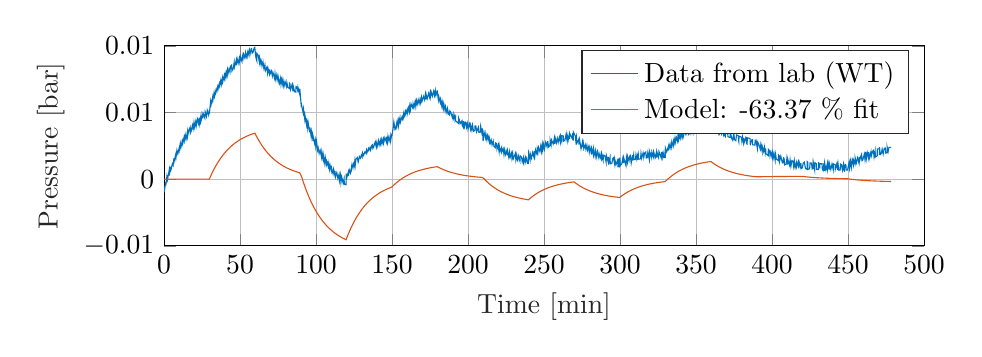
\begin{tikzpicture}

\begin{axis}[%
scaled y ticks = false,
 y tick label style={/pgf/number format/fixed,
/pgf/number format/1000 sep = \thinspace}, % Optional if you want to replace comma as the 1000 separator 
width=3.8in,
height=1in,
at={(1.011in,0.642in)},
scale only axis,
xmin=0,
xmax=500,
xlabel style={font=\color{white!15!black}},
xlabel={Time [min]},
ymin=-0.005,
ymax=0.01,
ylabel style={font=\color{white!15!black}},
ylabel={Pressure [bar]},
axis background/.style={fill=white},
%title style={font=\bfseries},
%title={Node WT},
xmajorgrids,
ymajorgrids,
legend style={legend cell align=left, align=left, draw=white!15!black}
]
\addplot [color=mycolor1]
  table[row sep=crcr]{%
0.000833333333333333	-0.000536486839485997\\
0.0508333333333333	-0.000992361717296275\\
1.07083333333333	-0.000214590456297223\\
1.15416666666667	-0.000472107562845242\\
1.86083333333333	0.000207354802741866\\
2.23	-4.84223233562925e-05\\
3.3075	0.000626690091107954\\
3.38583333333333	0.00026912410870214\\
4.09666666666667	0.000805908077422438\\
4.44416666666667	0.000669319612141839\\
5.46916666666667	0.00114433427489903\\
5.94	0.00103123554567336\\
6.4975	0.00157758940687817\\
6.65083333333333	0.00135139194838989\\
7.67916666666667	0.00184728637653113\\
7.8475	0.00162804883988631\\
8.4725	0.0021700527499505\\
9.06583333333333	0.00190383574114041\\
9.86583333333333	0.00231708109796219\\
10.0333333333333	0.00219441247628542\\
10.6625	0.00268682694352837\\
11.0708333333333	0.00237276047235473\\
11.9325	0.00287561482232949\\
12.2391666666667	0.00264245744206168\\
13.1041666666667	0.00312878197772765\\
13.3541666666667	0.00290519448994932\\
13.9108333333333	0.00333583965122845\\
14.45	0.00299306350267163\\
15.3741666666667	0.00356551707060934\\
15.4558333333333	0.00319925118595282\\
16.3025	0.00368905568249719\\
17.1833333333333	0.00390046330714998\\
17.2666666666667	0.00343501853685101\\
17.7641666666667	0.00356899703145931\\
18.6308333333333	0.00404227171378015\\
19.0908333333333	0.00377257474405045\\
19.6383333333333	0.00423018960235598\\
19.9341666666667	0.00388045353190596\\
20.8775	0.00436242811647393\\
21.1391666666667	0.00397441247625356\\
22.0441666666667	0.0044946666306203\\
22.67	0.00417973016928958\\
23.1425	0.00461211531109033\\
23.3208333333333	0.00417886017903019\\
24.1791666666667	0.00470868422599441\\
24.2483333333333	0.00433110846838648\\
25.3183333333333	0.00482178295526413\\
25.3691666666667	0.00455295597579951\\
25.79	0.0049087819777299\\
26.8133333333333	0.00458514561404404\\
27.0483333333333	0.0050358005505473\\
27.8891666666667	0.00470172430424899\\
28.3883333333333	0.00516716907457639\\
29.2941666666667	0.00481656301394655\\
29.7325	0.0051523792407011\\
29.7625	0.00490095206570235\\
30.6466666666667	0.00583619155747787\\
30.9566666666667	0.00560738412834215\\
31.9533333333333	0.00616591785262703\\
32.1408333333333	0.00594842029645977\\
32.8883333333333	0.00647563437269132\\
33.1991666666667	0.00620158745181247\\
34.0508333333333	0.00664006252517314\\
34.1708333333333	0.00652087386437759\\
35.2375	0.00694281912341242\\
35.4483333333333	0.00672184160628152\\
36.2408333333333	0.00713334698266412\\
36.4483333333333	0.00697674874195404\\
37.3158333333333	0.00742740367857099\\
37.6408333333333	0.00707940758862836\\
38.46	0.00757269204601703\\
38.6225	0.00731604492973477\\
39.6466666666667	0.00780062948502976\\
39.7975	0.00756138217316223\\
40.6383333333333	0.0079667976179849\\
40.7991666666667	0.00765708109780693\\
41.6566666666667	0.00818690514487348\\
41.8908333333333	0.00782411922099303\\
42.715	0.00827129419660654\\
43.3516666666667	0.00802073701192969\\
43.67	0.00845747210482846\\
44.3908333333333	0.0085496910686516\\
44.6391666666667	0.00811904590741509\\
45.4466666666667	0.00827303417712531\\
46.12	0.00876283867381748\\
46.3391666666667	0.0084157125740376\\
47.34	0.00886201755934056\\
47.4641666666667	0.00854534111753087\\
48.0433333333333	0.00904210553595707\\
48.7341666666667	0.00868540954363657\\
49.5266666666667	0.00909604492984502\\
49.745	0.00882373798954179\\
50.2425	0.00916390416738298\\
50.8483333333333	0.00889420719768171\\
51.74	0.00929005275006607\\
51.8875	0.00899686604425372\\
52.3775	0.00934312215351842\\
52.9958333333333	0.00912388461709955\\
53.6241666666667	0.0094927604723694\\
54.0066666666667	0.00912823456810659\\
55.0375	0.00955452977834743\\
55.165	0.0092430732779349\\
56.1508333333333	0.00968241834136736\\
56.4716666666667	0.00932572234918329\\
57.2933333333333	0.00978159722704962\\
57.5741666666667	0.0097902971291433\\
57.9783333333333	0.00945274092208596\\
58.5308333333333	0.00950929028662136\\
59.2725	0.0098451065133759\\
59.645	0.009886866044144\\
60.4433333333333	0.00909865490045834\\
61.0316666666667	0.00887158745175616\\
61.1091666666667	0.00942490123472912\\
61.9116666666667	0.00928483280862343\\
62.6825	0.0087697985954492\\
62.86	0.00909604492984502\\
63.8058333333333	0.00856796086343369\\
63.9925	0.00886897748114283\\
64.995	0.00851315147931477\\
65.1666666666667	0.00872716907451836\\
65.7458333333333	0.00828695402080944\\
66.3466666666667	0.00856883085373288\\
66.6825	0.00814340563367753\\
67.6433333333333	0.00840266272052763\\
68.0608333333333	0.00795896770581524\\
68.4358333333333	0.00827390416728808\\
69.1133333333333	0.00795374776472503\\
69.5491666666667	0.00822692469517965\\
69.5725	0.00784586897667626\\
70.65	0.00811034600502585\\
71.2266666666667	0.00772494033525394\\
71.6541666666667	0.00798419742237687\\
72.7375	0.00754050240778954\\
73.01	0.00791720817486526\\
73.6141666666667	0.00744828344392094\\
74.1575	0.00781106936782412\\
74.9383333333333	0.00738390416730685\\
75.115	0.00766665099071136\\
76.005	0.00719424629820654\\
76.65	0.00756399214379828\\
76.955	0.00711942713888906\\
77.415	0.00746307327787012\\
78.0891666666667	0.00708201755936673\\
78.2833333333333	0.00740913388382299\\
78.9216666666667	0.00695325900600215\\
79.5525	0.0073247448319876\\
80.4225	0.00694977904523743\\
80.7716666666667	0.00725253564354493\\
81.3908333333333	0.00688365978818413\\
82.4541666666667	0.00680275069711346\\
82.5333333333333	0.00718293642545408\\
82.8233333333333	0.00713421697295193\\
83.1758333333333	0.0067183616453463\\
84.1275	0.00706809771546664\\
84.8033333333333	0.00658960309225452\\
84.8933333333333	0.00701241834125317\\
85.9116666666667	0.0065565434635005\\
86.6733333333333	0.00652870377638241\\
86.8425	0.00695325900604761\\
87.67	0.00687843984666191\\
88.1383333333333	0.00650869400120659\\
88.2233333333333	0.0068323303650573\\
89.1141666666667	0.00642778491038602\\
89.2983333333333	0.0067879608633007\\
90.3308333333333	0.00538205665992568\\
90.4525	0.0055621446368264\\
91.4575	0.00500187093206254\\
91.7041666666667	0.00525851804817425\\
92.54	0.0045085864743783\\
92.7266666666667	0.00477045353203497\\
93.6683333333333	0.0041240507948601\\
93.8883333333333	0.00454947601482449\\
94.51	0.00382999409893049\\
94.8683333333333	0.00419104004230351\\
95.8275	0.00350983769623102\\
95.955	0.0038752335908271\\
96.76	0.00318794131306963\\
97.1091666666667	0.00357421697282238\\
98.0425	0.00285995499820051\\
98.1075	0.00319490123468999\\
99.0458333333333	0.00267899703131892\\
99.4766666666667	0.00293564414743062\\
99.8283333333333	0.0024319198074068\\
100.315833333333	0.00281993544775791\\
101.033333333333	0.00216657278884899\\
101.403333333333	0.00234405079478396\\
102.028333333333	0.00192471550636814\\
102.680833333333	0.00216396281815609\\
103.588333333333	0.001644578654134\\
103.755	0.00201258451930929\\
104.6	0.00147493056018679\\
104.76	0.00184032645473739\\
105.77	0.00114259429432199\\
106.074166666667	0.00161673896674305\\
106.840833333333	0.00112432449958537\\
107.080833333333	0.00133486213409245\\
107.939166666667	0.000972076210166539\\
108.080833333333	0.00118087386405254\\
108.774166666667	0.000732828898560495\\
109.131666666667	0.00108604492980934\\
110.001666666667	0.000624080120462653\\
110.216666666667	0.000841577676476427\\
111.150833333333	0.000406582564357938\\
111.563333333333	0.000743268781309356\\
112.415	0.000279563991478007\\
112.455833333333	0.000609290286672642\\
112.814166666667	0.000178645125436139\\
113.62	0.000489231635367599\\
114.365	4.81465916778168e-05\\
115.125833333333	0.000368302994468231\\
115.4075	-0.000117151550909925\\
116.065	0.00029870377637739\\
116.373333333333	-0.000248520074990169\\
116.908333333333	0.000155155389177292\\
117.788333333333	-0.000298109517950673\\
118.435	2.98767968957142e-05\\
118.604166666667	-0.000388588501198189\\
119.695833333333	-0.000419908149149217\\
119.880833333333	0.000413542486114735\\
120.1675	0.000105565946603325\\
121.139166666667	0.000501411498828513\\
121.283333333333	0.000227364577756392\\
121.854166666667	0.000693679338462552\\
122.6025	0.000460521958063995\\
123.380833333333	0.000961636327417678\\
123.4625	0.000743268781309356\\
124.504166666667	0.00114694424531767\\
124.9125	0.000882467217309155\\
125.5225	0.00139924141050191\\
125.796666666667	0.00107560504699226\\
126.219166666667	0.00148015050157259\\
127.1175	0.00161847894747784\\
127.699166666667	0.00128179273038999\\
128.011666666667	0.00140707132280798\\
128.468333333333	0.00170286799931323\\
129.098333333333	0.00156279957299152\\
129.788333333333	0.00180204688484768\\
130.3225	0.00165849849767032\\
130.539166666667	0.00198561482230847\\
131.248333333333	0.00178203710974006\\
132.12	0.0020352042650416\\
132.608333333333	0.00196995499810558\\
133.1375	0.00217962264219981\\
133.405833333333	0.0019525551938273\\
134.408333333333	0.00230316125424683\\
134.744166666667	0.00216309282819797\\
135.503333333333	0.00237363046250043\\
135.891666666667	0.00217788266171513\\
136.6675	0.00253457865395607\\
137.1925	0.00258851804782129\\
137.335833333333	0.00230490123493614\\
137.84	0.00238494033595775\\
138.808333333333	0.00276425607384002\\
139.506666666667	0.00246062948502872\\
139.593333333333	0.00275642616232975\\
140.186666666667	0.00245105959292008\\
140.965	0.00289475460775751\\
141.4925	0.00255110846823076\\
142.175833333333	0.00290171452942335\\
142.408333333333	0.00265115734435999\\
143.1275	0.00297740367904002\\
143.38	0.00266420719816556\\
144.2375	0.0030243831514213\\
144.466666666667	0.00270596672902461\\
145.256666666667	0.00311747210483876\\
146.374166666667	0.0027546861811857\\
146.4575	0.00318794131306963\\
147.056666666667	0.00280166565411268\\
147.330833333333	0.00322970084361035\\
148.071666666667	0.0028773548032746\\
148.791666666667	0.00325145059977107\\
149.050833333333	0.00287213486170688\\
149.860833333333	0.00340369888939453\\
149.893333333333	0.00325058060979021\\
150.83	0.0039135131604667\\
151.1775	0.00428847894744426\\
151.945	0.00371689536958687\\
152.315833333333	0.00378997454862433\\
153.1525	0.00426411922152287\\
153.238333333333	0.0039657125741883\\
154.2325	0.00442506741263746\\
154.315833333333	0.00405358158662925\\
155.198333333333	0.00460341540850781\\
155.4825	0.00426324923136011\\
156.505	0.00465735480250945\\
156.8	0.00451641638672985\\
157.609166666667	0.00493749165510739\\
157.6975	0.00461820524259342\\
158.700833333333	0.00503754053132756\\
158.765	0.00485658256478703\\
159.806666666667	0.00519326878155656\\
159.993333333333	0.00490617200701994\\
160.8075	0.0053516070025012\\
161.3525	0.00505581032551848\\
161.619166666667	0.00547688559498742\\
162.095833333333	0.00520022870363167\\
162.490833333333	0.00565175362988841\\
163.600833333333	0.00534203710998331\\
163.851666666667	0.00566654346388308\\
164.450833333333	0.00538466663091416\\
165.16	0.00582575167444478\\
165.6125	0.00545426584843657\\
166.054166666667	0.00589361091196002\\
166.581666666667	0.00563435382495077\\
167.184166666667	0.0059571201987524\\
167.7825	0.00566654346338287\\
168.3725	0.00599713974860382\\
168.805	0.00571700289646064\\
169.3875	0.00614677806805734\\
169.758333333333	0.00585620133305161\\
170.738333333333	0.00620854737334188\\
171.451666666667	0.00594059038461413\\
171.8825	0.00635209576097399\\
172.335833333333	0.00599365978804374\\
172.491666666667	0.00630511628886556\\
173.075833333333	0.00603280934827811\\
174.026666666667	0.00644257474422151\\
174.6175	0.00615721795001041\\
175.04	0.0064643245002458\\
175.360833333333	0.00618331765789439\\
175.693333333333	0.00655741345389065\\
176.583333333333	0.00622681716853325\\
177.395	0.00659917298493158\\
177.9325	0.00628684649394702\\
178.433333333333	0.00665920231057275\\
178.843333333333	0.0062868464943563\\
179.63	0.00661570279925176\\
179.706666666667	0.00660178295482867\\
180.4625	0.00593711042378121\\
180.76	0.00617635773527357\\
181.635833333333	0.00576311237872464\\
181.86	0.00597625998365177\\
182.786666666667	0.0054264261610911\\
183.0075	0.0058040019189662\\
183.839166666667	0.00530549752032815\\
184.069166666667	0.00563696379589378\\
184.88	0.00514367933859607\\
185.18	0.00543599605383636\\
186.074166666667	0.0049818611570004\\
186.4975	0.00529157767649625\\
187.1575	0.0048765923396218\\
187.725833333333	0.00480873310197015\\
188.004166666667	0.00511931961240183\\
188.5525	0.00504363046255779\\
189.555	0.00466518471465636\\
190.189166666667	0.00488964219260883\\
190.2725	0.00450249654303438\\
191.14	0.00476871355175494\\
191.398333333333	0.00445029712963109\\
191.813333333333	0.0046173352532492\\
191.844166666667	0.00437547797045003\\
193.7	0.00418147015033131\\
193.783333333333	0.00458949556563087\\
194.255	0.00444594717845352\\
194.815833333333	0.00417364023841177\\
195.985833333333	0.00437982792121833\\
196.06	0.00404836164551629\\
196.933333333333	0.00386914365898296\\
197.0175	0.00434067836112038\\
197.603333333333	0.00392917298521528\\
198.156666666667	0.00427629908507474\\
198.6375	0.00425802929006526\\
198.944166666667	0.00387784356206571\\
199.669166666667	0.00419191003314839\\
199.9775	0.0037664848125019\\
200.915	0.00414928051180827\\
201.564166666667	0.0037725747443233\\
201.768333333333	0.004033571811749\\
202.4675	0.00367687581978092\\
202.929166666667	0.00405184160612183\\
203.621666666667	0.00359161677714613\\
204.505	0.00365251609299552\\
204.585833333333	0.00399094229022698\\
205.1475	0.0039865923394132\\
205.626666666667	0.00354985724683278\\
206.756666666667	0.00389002342470807\\
207.026666666667	0.0035254975203657\\
207.9675	0.00351505763754861\\
208.286666666667	0.00395875265261342\\
209.04	0.00348634796044965\\
209.41	0.00380650436303544\\
209.411666666667	0.003812594294584\\
209.891666666667	0.00285473505736039\\
210.5625	0.00350287777404222\\
211.525833333333	0.00307745255462354\\
211.723333333333	0.00338542909456695\\
212.393333333333	0.00294173407995689\\
212.790833333333	0.00327059038417023\\
213.818333333333	0.00284951511602007\\
213.905833333333	0.00311660211476696\\
214.634166666667	0.00270422674806245\\
215.219166666667	0.00293738412837005\\
215.784166666667	0.00256589830254374\\
216.515833333333	0.00286343495948817\\
217.0375	0.00246323945660837\\
217.864166666667	0.00236145059951699\\
218.144166666667	0.0027146666312888\\
218.6975	0.00267116712001329\\
219.034166666667	0.00225009185086268\\
219.7325	0.00253892860536102\\
220.304166666667	0.0021256832485847\\
220.466666666667	0.00253805861560753\\
221.120833333333	0.00209610358141393\\
222.034166666667	0.00237015050169025\\
222.084166666667	0.00201867445101701\\
223.091666666667	0.0022883714202067\\
223.623333333333	0.0018377164846584\\
224.093333333333	0.0022266021144674\\
224.74	0.00184206643579049\\
225.549166666667	0.00215091296530549\\
225.881666666667	0.00178029712923265\\
226.07	0.00207783378617708\\
226.785833333333	0.00165066858606909\\
227.296666666667	0.00204651413822607\\
227.7325	0.0016463186351189\\
228.655833333333	0.00197256496916229\\
228.861666666667	0.00160542909446808\\
229.399166666667	0.00192471550730038\\
229.7125	0.00151495011044749\\
231.155	0.00193602537959808\\
231.414166666667	0.00150712019839151\\
231.775833333333	0.00181248676798308\\
232.34	0.00143404101949049\\
232.639166666667	0.00137227171379667\\
232.999166666667	0.00178029712941456\\
234.129166666667	0.00135574189988578\\
234.308333333333	0.00173940758867279\\
235.156666666667	0.00166371843987466\\
235.661666666667	0.00129484258380902\\
236.54	0.00165414854672012\\
236.575	0.00123481325857715\\
237.670833333333	0.0016002091528549\\
237.693333333333	0.00126178295512322\\
238.505	0.00155931961184028\\
239.070833333333	0.00119044375650222\\
239.6075	0.00117391394240944\\
239.890833333333	0.00195429517460756\\
240.770833333333	0.00144361091214482\\
240.981666666667	0.00188034600531641\\
241.724166666667	0.00157149947530119\\
242.4275	0.00199170475401619\\
243.393333333333	0.00162021892778061\\
243.575833333333	0.00209262362021721\\
243.964166666667	0.00176898725625282\\
244.370833333333	0.00219876242762215\\
245.205	0.00190557572271931\\
245.478333333333	0.00228489146019233\\
245.949166666667	0.00199866467600035\\
246.354166666667	0.0023849403364125\\
247.235	0.00207261384506413\\
247.829166666667	0.00248933916312812\\
248.329166666667	0.00208044375707463\\
248.8375	0.00259895793068385\\
249.189166666667	0.00220050240808409\\
249.7075	0.00261461775579623\\
250.246666666667	0.00224835187026433\\
251.099166666667	0.002765996054211\\
251.9675	0.00242582987633572\\
252.328333333333	0.00280775558525197\\
252.44	0.00281210553670239\\
253.056666666667	0.00240843007194375\\
253.8975	0.0025180488399997\\
253.983333333333	0.00291563437293693\\
254.624166666667	0.00255023847834085\\
254.914166666667	0.00293651413852562\\
255.990833333333	0.00264158745266062\\
256.754166666667	0.00305570279941779\\
256.984166666667	0.0026502873544246\\
257.270833333333	0.0031157321244223\\
258.0975	0.00271988657240176\\
258.724166666667	0.00306875265308694\\
259.311666666667	0.00276686604410091\\
260.065833333333	0.00315053173316077\\
260.6775	0.00278165587832295\\
260.901666666667	0.00321230103949123\\
261.615833333333	0.0028521250865538\\
261.699166666667	0.0032523205899793\\
262.6825	0.00324884062919185\\
262.825	0.00284429517467974\\
263.676666666667	0.00289301462684083\\
264.419166666667	0.00332017982713072\\
265.101666666667	0.00291911433363343\\
265.186666666667	0.00331930983696797\\
265.890833333333	0.00294956399196739\\
266.551666666667	0.00336280934869823\\
266.7825	0.00302699312186409\\
266.865	0.00341587875230974\\
268.590833333333	0.00303569302376448\\
268.773333333333	0.00344545841975336\\
269.238333333333	0.00289997454923427\\
269.3225	0.00351418764734039\\
270.565	0.00322883085349307\\
270.881666666667	0.00287735480300175\\
271.269166666667	0.00315053173366099\\
271.513333333333	0.00268073701262214\\
272.8425	0.00299828344431038\\
272.875833333333	0.00259547797007829\\
273.335833333333	0.00296000387442068\\
274.323333333333	0.00228402146984767\\
275.316666666667	0.00281123554599393\\
275.539166666667	0.00238494033577584\\
275.8475	0.00265376731539395\\
276.171666666667	0.00227793153734414\\
277.071666666667	0.00258764805674903\\
277.536666666667	0.00224139194777993\\
278.160833333333	0.00254066858495892\\
278.6025	0.00216570279816328\\
279.3575	0.00243539976671631\\
279.738333333333	0.00203607425481782\\
280.2075	0.00237102049085255\\
281.035833333333	0.00195429517324332\\
281.131666666667	0.00184293642504375\\
281.3275	0.00231447112599885\\
282.463333333333	0.00179769693339725\\
282.5475	0.00229533134150874\\
283.586666666667	0.00171765783314871\\
283.935	0.00211872332555461\\
284.645	0.00166284844871147\\
285.168333333333	0.00209871355162936\\
285.479166666667	0.00199083476344417\\
286.078333333333	0.00159150925018142\\
286.728333333333	0.00191253564133835\\
287.343333333333	0.00153669986619892\\
287.755833333333	0.00145057083344685\\
287.929166666667	0.00191340563295629\\
288.8725	0.00142099116554849\\
289.056666666667	0.00180291687473759\\
289.9725	0.00175854737252625\\
290.835833333333	0.00126526291604709\\
290.9875	0.0017776871578349\\
292.059166666667	0.00133486213416066\\
292.293333333333	0.00166458842949173\\
292.654166666667	0.00127396281831128\\
293.415833333333	0.00162891882945364\\
293.560833333333	0.00114694424554504\\
294.574166666667	0.00117130397237591\\
295.185833333333	0.00154539976864503\\
295.633333333333	0.00160281912347958\\
296.4	0.00115564414871873\\
296.49	0.00151234013973184\\
297.338333333333	0.00109822479324752\\
298.370833333333	0.00142012117556764\\
298.639166666667	0.000892907099921597\\
298.723333333333	0.00154191980699356\\
299.735	0.000878987257226557\\
299.818333333333	0.00160716907402052\\
300.2225	0.00102775558533498\\
301.149166666667	0.0011573841273162\\
301.861666666667	0.00158628930829539\\
302.311666666667	0.00121045353261028\\
302.393333333333	0.00160803906418326\\
303.900833333333	0.00101470573289365\\
304.184166666667	0.00165153857586806\\
304.766666666667	0.00129310260289234\\
304.9575	0.00169938803782092\\
305.860833333333	0.00135835187073784\\
306.335	0.00171765783287586\\
306.685	0.00177681716739929\\
307.318333333333	0.0012121935118444\\
308.164166666667	0.00179334698231064\\
308.2475	0.00138619155803785\\
308.95	0.00183597650328697\\
309.165833333333	0.00146362068779812\\
310.108333333333	0.00147145059880817\\
310.474166666667	0.00184119644417255\\
311.023333333333	0.00149929028583533\\
311.6425	0.00185511628759517\\
311.924166666667	0.00194907523108444\\
311.993333333333	0.00149059038329828\\
313.476666666667	0.00152712997440861\\
313.768333333333	0.00192645548603426\\
314.201666666667	0.00156366956369997\\
315.143333333333	0.00196299507532562\\
315.601666666667	0.00162717884885527\\
316.098333333333	0.00196038510520115\\
316.8975	0.00203520426520075\\
317.2575	0.00158628930820445\\
317.854166666667	0.00161151902501619\\
318.255833333333	0.00198648481226658\\
319.21	0.0014862404323026\\
319.298333333333	0.00210306350171553\\
320.500833333333	0.00161412899568635\\
320.69	0.00200040465523448\\
320.839166666667	0.00163413877115776\\
320.9175	0.00203172430291264\\
322.065833333333	0.0016323987901956\\
322.149166666667	0.00202824434244352\\
323.178333333333	0.0016323987898318\\
323.925833333333	0.00202998432267808\\
324.149166666667	0.00160890905507362\\
324.2325	0.00203694424443487\\
325.323333333333	0.0016332687808131\\
325.594166666667	0.00206739390258694\\
327.071666666667	0.00159498921119625\\
327.155	0.00198735480115605\\
327.753333333333	0.00201780445994476\\
328.114166666667	0.00161064903530818\\
328.758333333333	0.00196473505583303\\
329.06	0.00163413877170346\\
329.755	0.00162717884949191\\
329.841666666667	0.00232839097042191\\
330.665	0.00204042420526779\\
331.738333333333	0.00244322967936345\\
331.764166666667	0.00213786311013568\\
332.288333333333	0.00259199800801756\\
332.9175	0.00232143104730088\\
333.6775	0.00275903613190852\\
333.9975	0.00239712019846369\\
335.015833333333	0.00287735480150107\\
335.255	0.00256241834084679\\
336.065	0.00306614268118896\\
336.334166666667	0.00272945646373732\\
337.068333333333	0.0031218220560618\\
337.800833333333	0.00284603515455049\\
338.108333333333	0.00326972039355272\\
338.54	0.00297392371793424\\
338.9075	0.00332626975831549\\
339.575833333333	0.00305570279878115\\
340.0975	0.00345241834173753\\
340.745	0.0031018122809542\\
341.628333333333	0.00351853759838154\\
341.668333333333	0.00322361091210727\\
342.7225	0.00372472528223401\\
343.404166666667	0.00327842029518027\\
343.478333333333	0.00369775558482392\\
344.9075	0.00385522381501463\\
344.936666666667	0.00334714952322206\\
345.384166666667	0.00341065881128774\\
345.468333333333	0.00383434405047187\\
346.135	0.00347764805718502\\
346.8675	0.00392569302374572\\
347.3175	0.00354463730471938\\
348.179166666667	0.00405793153785229\\
348.426666666667	0.00359596672832371\\
349.1075	0.00407881130266791\\
349.726666666667	0.00408403124555438\\
349.755	0.00358552684637065\\
350.864166666667	0.00372646526310522\\
351.400833333333	0.00421452977860785\\
352.269166666667	0.00420930983772226\\
352.418333333333	0.00383434404983522\\
352.825833333333	0.00424323945752579\\
353.6225	0.00383173408025644\\
354.305	0.00387436360050518\\
354.7875	0.00436938803812841\\
355.030833333333	0.00381607425496217\\
355.1125	0.00431283867336564\\
356.963333333333	0.00396136262323811\\
357.045833333333	0.00438939781460025\\
357.815	0.00399094229086362\\
357.995	0.00430152880052223\\
358.451666666667	0.00446247699209155\\
358.741666666667	0.00388915343381772\\
359.403333333333	0.00435894815517489\\
360.095833333333	0.00387523359048604\\
360.716666666667	0.00424671941672163\\
361.505	0.00375343495860538\\
361.5725	0.00413623066004906\\
362.488333333333	0.00373516516364138\\
362.871666666667	0.00404836164442489\\
363.680833333333	0.00363424629866817\\
364.046666666667	0.00395179273081116\\
364.771666666667	0.00352114756841505\\
365.053333333333	0.00385696379606774\\
365.450833333333	0.0034759080768595\\
366.105833333333	0.00382912410813109\\
366.700833333333	0.0034411084688941\\
367.151666666667	0.00373429517438811\\
368.115	0.00331582987581673\\
368.621666666667	0.00364642616312953\\
368.876666666667	0.00324797063848341\\
369.27	0.00319142127372064\\
369.4375	0.0036029266504443\\
370.769166666667	0.00352375754008566\\
370.985	0.00317576144869922\\
372.423333333333	0.00312791198711014\\
372.441666666667	0.00346720817532291\\
372.683333333333	0.003493307881206\\
373.478333333333	0.00303830299334326\\
374.13	0.00291041442995951\\
374.654166666667	0.00335671941683134\\
375.045	0.0033193098361949\\
375.143333333333	0.00298001364889164\\
376.146666666667	0.00288692469529227\\
376.610833333333	0.00331756985668794\\
377.888333333333	0.00324623065715744\\
378.021666666667	0.00287039488092664\\
378.129166666667	0.00280775558429699\\
378.280833333333	0.00321752097996754\\
379.829166666667	0.003156621664391\\
380.155	0.0028442951733155\\
380.603333333333	0.00317315147848379\\
381.168333333333	0.00276686604310047\\
381.405	0.0031018122811361\\
381.488333333333	0.00268508696225357\\
382.704166666667	0.00310355226073401\\
383.408333333333	0.00262853759767272\\
383.6025	0.00262157767591592\\
383.683333333333	0.003100072300083\\
385.525833333333	0.00305222283658399\\
385.653333333333	0.00261983769549946\\
385.7975	0.00260156790044451\\
386.628333333333	0.00294086408829347\\
387.2225	0.0029713137461727\\
387.245833333333	0.00257111824292909\\
388.753333333333	0.00255632840861612\\
388.846666666667	0.00292172430425812\\
389.454166666667	0.00293042420597661\\
390.058333333333	0.00246236946439925\\
390.344166666667	0.00228750142931634\\
390.585833333333	0.00277469595411052\\
391.265833333333	0.00261200778385277\\
392.271666666667	0.00223965196654494\\
392.604166666667	0.0025980879401573\\
393.464166666667	0.00208392371695258\\
393.544166666667	0.00245714952433222\\
394.4	0.00207783378581329\\
394.961666666667	0.00241538999315484\\
395.445	0.00197430494844188\\
395.774166666667	0.00230403124286344\\
395.988333333333	0.00190818569152501\\
397.4675	0.00176637728453674\\
397.545	0.00223791198585563\\
398.365	0.00212568324803901\\
398.661666666667	0.00173940758839994\\
399.241666666667	0.00203259429425774\\
400.021666666667	0.00160716907438431\\
400.294166666667	0.00197343495837007\\
400.805833333333	0.00162108891880738\\
401.275	0.00194820524237688\\
402.045	0.00140011140055098\\
402.3325	0.00184467640555117\\
402.779166666667	0.00151495011040201\\
404.080833333333	0.0013975014307903\\
404.159166666667	0.00181944668919418\\
404.886666666667	0.00171765783269397\\
404.919166666667	0.00132181228090079\\
405.76	0.00172287777476189\\
406.674166666667	0.00126178295557797\\
407.135833333333	0.00121306350200716\\
407.583333333333	0.00159933916237381\\
407.891666666667	0.00157845939619396\\
408.323333333333	0.00107212508572734\\
409.380833333333	0.00114172430438661\\
409.74	0.0015497497203683\\
410.174166666667	0.00109300485127055\\
410.255833333333	0.00151930006176147\\
411.514166666667	0.00104776536089733\\
411.856666666667	0.00143926096042155\\
412.4075	0.000963376307379388\\
412.975	0.00138706154747301\\
413.7275	0.0013600918509724\\
414.178333333333	0.000969466240519565\\
414.638333333333	0.0013766216645195\\
415.12	0.000898127042353314\\
416.009166666667	0.00123655323931192\\
416.031666666667	0.000892907100285389\\
417.148333333333	0.00130615245651601\\
417.5325	0.000813737990108657\\
417.906666666667	0.00125482303282073\\
418.781666666667	0.000898127041443819\\
418.910833333333	0.00120088363991049\\
419.2925	0.000810258028275293\\
419.920833333333	0.000842447666570975\\
420.500833333333	0.00120523359145185\\
421.184166666667	0.00128092274097756\\
421.975833333333	0.000805038087116863\\
423.079166666667	0.000730218927844847\\
423.163333333333	0.00130615245769836\\
423.4575	0.00127048285738741\\
423.511666666667	0.000734568878203876\\
424.706666666667	0.000770238478514818\\
425.04	0.00122263339470695\\
425.976666666667	0.00120523359054235\\
426.383333333333	0.000762408566322426\\
427.003333333333	0.000799818146413181\\
427.086666666667	0.00128092273979523\\
428.054166666667	0.000677149524096907\\
428.233333333333	0.00123220328749771\\
429.253333333333	0.00115042420601416\\
429.2825	0.000734568879386222\\
430.565833333333	0.000720649036782137\\
430.65	0.00127483280920164\\
431.350833333333	0.000810258029002892\\
431.44	0.00115129419672261\\
432.860833333333	0.00115129419745021\\
432.979166666667	0.000792858224565443\\
433.5375	0.000658009738606358\\
434.141666666667	0.00119305372671764\\
434.469166666667	0.000626690091110091\\
434.551666666667	0.00121828344452983\\
435.449166666667	0.000704119222234609\\
436.378333333333	0.00117391394231849\\
436.495	0.000732828899333557\\
437.1925	0.00115303417741192\\
437.654166666667	0.000722389015561514\\
437.729166666667	0.0011686940016148\\
438.663333333333	0.000723259007543262\\
439.4075	0.00113041443217984\\
440.228333333333	0.000704989211942605\\
440.310833333333	0.00114955421539666\\
441.473333333333	0.00108952489116522\\
441.593333333333	0.000740658811344053\\
442.635833333333	0.00117652391389815\\
443.065833333333	0.000683239456509485\\
443.431666666667	0.00112084454057143\\
443.889166666667	0.000672799573919788\\
444.8	0.000685849426633953\\
444.981666666667	0.00113215441214155\\
445.685	0.0010860449301504\\
446.265	0.000676279533661311\\
446.933333333333	0.00110170475380759\\
447.2425	0.000629300061598351\\
447.55	0.000609290286399791\\
448.026666666667	0.00110953466618188\\
448.576666666667	0.00107995499828352\\
448.758333333333	0.000679759495221824\\
449.6825	0.000686719417615264\\
450.643333333333	0.00124351316097776\\
450.9575	0.000830267804019555\\
451.579166666667	0.00136879175250901\\
452.1425	0.000876377285192159\\
452.709166666667	0.00144100094092896\\
453.4975	0.00107821501759421\\
453.575833333333	0.00143143104877484\\
454.539166666667	0.00112171452936995\\
454.62	0.00162108891762504\\
455.485833333333	0.00121480348251456\\
456.2475	0.00159933916146432\\
457.2025	0.00118870377635862\\
457.3875	0.00165936848769664\\
457.511666666667	0.00132181228080984\\
458.450833333333	0.0017515874508604\\
458.930833333333	0.00187251609276022\\
459.0675	0.00138271159620448\\
459.643333333333	0.00142012117520383\\
460.675833333333	0.0018690361317454\\
461.1	0.00149233036398759\\
461.5725	0.00204564414724477\\
461.985	0.00150886017862607\\
462.648333333333	0.001986484811539\\
463.486666666667	0.00156714952453289\\
463.569166666667	0.00202128442050484\\
464.115	0.00161064903539913\\
465.079166666667	0.00205695402054293\\
465.31	0.00174027757828985\\
466.140833333333	0.00208392371740733\\
466.655	0.00214134307124145\\
467.113333333333	0.00168024825196657\\
467.778333333333	0.00214047308171533\\
468.005	0.00165762850737114\\
469.170833333333	0.00175506741151142\\
469.253333333333	0.00226401169364866\\
470.563333333333	0.00227184160529535\\
470.586666666667	0.00182118666897399\\
470.67	0.00239538021768343\\
471.190833333333	0.00184119644517299\\
471.875833333333	0.00191253564261164\\
472.42	0.0022535718107861\\
473.109166666667	0.00188991589719766\\
473.813333333333	0.00233013095083838\\
474.513333333333	0.00233274092069\\
474.81	0.00195429517433471\\
475.64	0.00199083476271657\\
475.723333333333	0.00239538021795628\\
476.329166666667	0.00204564414597147\\
476.949166666667	0.00238581032543837\\
478.334166666667	0.00238320035404062\\
};
\addlegendentry{Data from lab (WT)}

\addplot [color=mycolor2]
  table[row sep=crcr]{%
0.000833333333333333	0\\
0.000833333333333333	0\\
1.10333333333333	-5.06498171062578e-16\\
1.10333333333333	-5.06498171062578e-16\\
2.20583333333333	-9.76845476540721e-16\\
2.20583333333333	-9.76845476540721e-16\\
3.3075	-1.41330407548488e-15\\
3.3075	-1.41330407548488e-15\\
4.41	-1.81892889974846e-15\\
4.41	-1.81892889974846e-15\\
5.51166666666667	-2.19532829745552e-15\\
5.51166666666667	-2.19532829745552e-15\\
6.61416666666667	-2.54513682435173e-15\\
6.61416666666667	-2.54513682435173e-15\\
7.71666666666667	-2.86997807247266e-15\\
7.71666666666667	-2.86997807247266e-15\\
8.81833333333333	-3.17141438215868e-15\\
8.81833333333333	-3.17141438215868e-15\\
9.92083333333333	-3.45155561534515e-15\\
9.92083333333333	-3.45155561534515e-15\\
11.0225	-3.71151256358124e-15\\
11.0225	-3.71151256358124e-15\\
12.125	-3.95310475972428e-15\\
12.125	-3.95310475972428e-15\\
13.2266666666667	-4.17729014404833e-15\\
13.2266666666667	-4.17729014404833e-15\\
14.3291666666667	-4.38563787127583e-15\\
14.3291666666667	-4.38563787127583e-15\\
15.4316666666667	-4.57911496103191e-15\\
15.4316666666667	-4.57911496103191e-15\\
16.5333333333333	-4.75865195112238e-15\\
16.5333333333333	-4.75865195112238e-15\\
17.6358333333333	-4.92550548598326e-15\\
17.6358333333333	-4.92550548598326e-15\\
18.7375	-5.08033715867713e-15\\
18.7375	-5.08033715867713e-15\\
19.84	-5.22423069217336e-15\\
19.84	-5.22423069217336e-15\\
20.9425	-5.35785395010874e-15\\
20.9425	-5.35785395010874e-15\\
22.0441666666667	-5.48184960027095e-15\\
22.0441666666667	-5.48184960027095e-15\\
23.1466666666667	-5.59708553313643e-15\\
23.1466666666667	-5.59708553313643e-15\\
24.2483333333333	-5.70401867216091e-15\\
24.2483333333333	-5.70401867216091e-15\\
25.3508333333333	-5.80339748112399e-15\\
25.3508333333333	-5.80339748112399e-15\\
26.4525	-5.89561600819868e-15\\
26.4525	-5.89561600819868e-15\\
27.555	-5.98131972426477e-15\\
27.555	-5.98131972426477e-15\\
28.6575	-6.06090641228102e-15\\
29.7525	-6.13432816906353e-15\\
29.7591666666667	1.78270662453254e-06\\
29.7591666666667	1.78270662453254e-06\\
30.8616666666667	0.00028588328038675\\
30.8616666666667	0.00028588328038675\\
31.9633333333333	0.000549514297167854\\
31.9633333333333	0.000549514297167854\\
33.0658333333333	0.000794521005962208\\
33.0658333333333	0.000794521005962208\\
34.1675	0.00102187488597133\\
34.1675	0.00102187488597133\\
35.27	0.00123316726936686\\
35.27	0.00123316726936686\\
36.3725	0.00142937884302303\\
36.3725	0.00142937884302303\\
37.4741666666667	0.00161145329638366\\
37.4741666666667	0.00161145329638366\\
38.5766666666667	0.00178066503450945\\
38.5766666666667	0.00178066503450945\\
39.6783333333333	0.00193768500100462\\
39.6783333333333	0.00193768500100462\\
40.7808333333333	0.00208361223549934\\
40.7808333333333	0.00208361223549934\\
41.8833333333333	0.00221912404079664\\
41.8833333333333	0.00221912404079664\\
42.985	0.00234487216774788\\
42.985	0.00234487216774788\\
44.0875	0.0024617367730494\\
44.0875	0.0024617367730494\\
45.1891666666667	0.00257018123802662\\
45.1891666666667	0.00257018123802662\\
46.2916666666667	0.00267096460477698\\
46.2916666666667	0.00267096460477698\\
47.3933333333333	0.0027644864907034\\
47.3933333333333	0.0027644864907034\\
48.4958333333333	0.00285140148936645\\
48.4958333333333	0.00285140148936645\\
49.5983333333333	0.00293211300573982\\
49.5983333333333	0.00293211300573982\\
50.7	0.0030070092259258\\
50.7	0.0030070092259258\\
51.8025	0.00307661437570275\\
51.8025	0.00307661437570275\\
52.9041666666667	0.00314120444733089\\
52.9041666666667	0.00314120444733089\\
54.0066666666667	0.00320123153012113\\
54.0066666666667	0.00320123153012113\\
55.1091666666667	0.00325697423218633\\
55.1091666666667	0.00325697423218633\\
56.2108333333333	0.00330870065085902\\
56.2108333333333	0.00330870065085902\\
57.3133333333333	0.00335677283808284\\
57.3133333333333	0.00335677283808284\\
58.415	0.00340138140549572\\
58.415	0.00340138140549572\\
59.5175	0.00344283858462169\\
59.7525	0.00345128528891706\\
60.6191666666667	0.00325612258718831\\
60.6191666666667	0.00325612258718831\\
61.7216666666667	0.00302371967499423\\
61.7216666666667	0.00302371967499423\\
62.8241666666667	0.00280790431813626\\
62.8241666666667	0.00280790431813626\\
63.9258333333333	0.0026076385417881\\
63.9258333333333	0.0026076385417881\\
65.0283333333333	0.00242152061322916\\
65.0283333333333	0.00242152061322916\\
66.13	0.00224881255390558\\
66.13	0.00224881255390558\\
67.2325	0.00208830551754178\\
67.2325	0.00208830551754178\\
68.3341666666667	0.00193936307565667\\
68.3341666666667	0.00193936307565667\\
69.4366666666667	0.00180094272614111\\
69.4366666666667	0.00180094272614111\\
70.5391666666667	0.00167240200844926\\
70.5391666666667	0.00167240200844926\\
71.6408333333333	0.00155312269952663\\
71.6408333333333	0.00155312269952663\\
72.7433333333333	0.00144226992027778\\
72.7433333333333	0.00144226992027778\\
73.845	0.00133940412694488\\
73.845	0.00133940412694488\\
74.9475	0.00124380532457432\\
74.9475	0.00124380532457432\\
76.05	0.00115502980341576\\
76.05	0.00115502980341576\\
77.1516666666667	0.00107265059312985\\
77.1516666666667	0.00107265059312985\\
78.2541666666667	0.000996091091779613\\
78.2541666666667	0.000996091091779613\\
79.3558333333333	0.000925047732317266\\
79.3558333333333	0.000925047732317266\\
80.4583333333333	0.000859023256532542\\
80.4583333333333	0.000859023256532542\\
81.56	0.000797755869941008\\
81.56	0.000797755869941008\\
82.6625	0.000740816739908063\\
82.6625	0.000740816739908063\\
83.765	0.00068794159066303\\
83.765	0.00068794159066303\\
84.8666666666667	0.000638876116513063\\
84.8666666666667	0.000638876116513063\\
85.9691666666667	0.000593276890429228\\
85.9691666666667	0.000593276890429228\\
87.0708333333333	0.000550963106343122\\
87.0708333333333	0.000550963106343122\\
88.1733333333333	0.000511638594750564\\
88.1733333333333	0.000511638594750564\\
89.2758333333333	0.000475120835904502\\
89.2758333333333	0.000475120835904502\\
90.3775	0.000222959404430519\\
90.3775	0.000222959404430519\\
91.48	-0.00017192454596155\\
91.48	-0.00017192454596155\\
92.5816666666667	-0.00053835695394235\\
92.5816666666667	-0.00053835695394235\\
93.6841666666667	-0.000878902612685697\\
93.6841666666667	-0.000878902612685697\\
94.7858333333333	-0.00119491182409279\\
94.7858333333333	-0.00119491182409279\\
95.8883333333333	-0.00148859645111756\\
95.8883333333333	-0.00148859645111756\\
96.9908333333333	-0.0017613195938126\\
96.9908333333333	-0.0017613195938126\\
98.0925	-0.00201439292786573\\
98.0925	-0.00201439292786573\\
99.195	-0.00224958780522486\\
99.195	-0.00224958780522486\\
100.296666666667	-0.00246783680007479\\
100.296666666667	-0.00246783680007479\\
101.399166666667	-0.00267066751619737\\
101.399166666667	-0.00267066751619737\\
102.500833333333	-0.00285888420023192\\
102.500833333333	-0.00285888420023192\\
103.603333333333	-0.00303380424893682\\
103.603333333333	-0.00303380424893682\\
104.705833333333	-0.00319623953159513\\
104.705833333333	-0.00319623953159513\\
105.8075	-0.0033469712888783\\
105.8075	-0.0033469712888783\\
106.91	-0.00348705454696242\\
106.91	-0.00348705454696242\\
108.011666666667	-0.00361704475174686\\
108.011666666667	-0.00361704475174686\\
109.114166666667	-0.00373785175176753\\
109.114166666667	-0.00373785175176753\\
110.216666666667	-0.00385003625743598\\
110.216666666667	-0.00385003625743598\\
111.318333333333	-0.0039541378257816\\
111.318333333333	-0.0039541378257816\\
112.420833333333	-0.00405088510139495\\
112.420833333333	-0.00405088510139495\\
113.5225	-0.00414066169812264\\
113.5225	-0.00414066169812264\\
114.625	-0.00422409599488925\\
114.625	-0.00422409599488925\\
115.726666666667	-0.00430151881808078\\
115.726666666667	-0.00430151881808078\\
116.829166666667	-0.00437347207808531\\
116.829166666667	-0.00437347207808531\\
117.931666666667	-0.00444028973685892\\
117.931666666667	-0.00444028973685892\\
119.033333333333	-0.00450229315729608\\
119.7525	-0.00454036306865793\\
120.135833333333	-0.00442495637971615\\
120.135833333333	-0.00442495637971615\\
121.2375	-0.00410935897172602\\
121.2375	-0.00410935897172602\\
122.34	-0.00381605705611791\\
122.34	-0.00381605705611791\\
123.4425	-0.00354368930914605\\
123.4425	-0.00354368930914605\\
124.544166666667	-0.00329094576441576\\
124.544166666667	-0.00329094576441576\\
125.646666666667	-0.00305605737829397\\
125.646666666667	-0.00305605737829397\\
126.748333333333	-0.00283809279186834\\
126.748333333333	-0.00283809279186834\\
127.850833333333	-0.00263552639203466\\
127.850833333333	-0.00263552639203466\\
128.9525	-0.00244755498019746\\
128.9525	-0.00244755498019746\\
130.055	-0.00227286287634732\\
130.055	-0.00227286287634732\\
131.1575	-0.0021106392691784\\
131.1575	-0.0021106392691784\\
132.259166666667	-0.00196010393608316\\
132.259166666667	-0.00196010393608316\\
133.361666666667	-0.00182020322572934\\
133.361666666667	-0.00182020322572934\\
134.463333333333	-0.00169038241604012\\
134.463333333333	-0.00169038241604012\\
135.565833333333	-0.00156973284413723\\
135.565833333333	-0.00156973284413723\\
136.6675	-0.00145777612087632\\
136.6675	-0.00145777612087632\\
137.77	-0.00135372862059179\\
137.77	-0.00135372862059179\\
138.8725	-0.00125710741997046\\
138.8725	-0.00125710741997046\\
139.974166666667	-0.00116744781448254\\
139.974166666667	-0.00116744781448254\\
141.076666666667	-0.00108412224406748\\
141.076666666667	-0.00108412224406748\\
142.178333333333	-0.00100680031345155\\
142.178333333333	-0.00100680031345155\\
143.280833333333	-0.000934940818430394\\
143.280833333333	-0.000934940818430394\\
144.383333333333	-0.000868210232246258\\
144.383333333333	-0.000868210232246258\\
145.485	-0.000806287610784579\\
145.485	-0.000806287610784579\\
146.5875	-0.000748739535184527\\
146.5875	-0.000748739535184527\\
147.689166666667	-0.000695337820843266\\
147.689166666667	-0.000695337820843266\\
148.791666666667	-0.00064570868981584\\
148.791666666667	-0.00064570868981584\\
149.893333333333	-0.000588597916562289\\
149.893333333333	-0.000588597916562289\\
150.995833333333	-0.000462757198926377\\
150.995833333333	-0.000462757198926377\\
152.098333333333	-0.000345898252851074\\
152.098333333333	-0.000345898252851074\\
153.2	-0.000237459039350626\\
153.2	-0.000237459039350626\\
154.3025	-0.000136680553084567\\
154.3025	-0.000136680553084567\\
155.404166666667	-4.3163196001626e-05\\
155.404166666667	-4.3163196001626e-05\\
156.506666666667	4.37475937596935e-05\\
156.506666666667	4.37475937596935e-05\\
157.609166666667	0.000124455201638058\\
157.609166666667	0.000124455201638058\\
158.710833333333	0.000199347794937586\\
158.710833333333	0.000199347794937586\\
159.813333333333	0.000268949574050775\\
159.813333333333	0.000268949574050775\\
160.915	0.000333536517872797\\
160.915	0.000333536517872797\\
162.0175	0.000393560693821909\\
162.0175	0.000393560693821909\\
163.119166666667	0.000449260104517776\\
163.119166666667	0.000449260104517776\\
164.221666666667	0.000501024610314581\\
164.221666666667	0.000501024610314581\\
165.324166666667	0.000549094469619133\\
165.324166666667	0.000549094469619133\\
166.425833333333	0.000593700876840227\\
166.425833333333	0.000593700876840227\\
167.528333333333	0.000635156048381938\\
167.528333333333	0.000635156048381938\\
168.63	0.00067362435866956\\
168.63	0.00067362435866956\\
169.7325	0.00070937506134303\\
169.7325	0.00070937506134303\\
170.834166666667	0.000742549911965946\\
170.834166666667	0.000742549911965946\\
171.936666666667	0.000773381113336346\\
171.936666666667	0.000773381113336346\\
173.039166666667	0.000802011764576018\\
173.039166666667	0.000802011764576018\\
174.140833333333	0.000828579566243808\\
174.140833333333	0.000828579566243808\\
175.243333333333	0.000853270476008528\\
175.243333333333	0.000853270476008528\\
176.345	0.000876182396108951\\
176.345	0.000876182396108951\\
177.4475	0.000897475695374347\\
177.4475	0.000897475695374347\\
178.55	0.000917249203960192\\
178.55	0.000917249203960192\\
179.651666666667	0.000935598023551736\\
179.7525	0.000937210620107562\\
180.754166666667	0.000876232231005131\\
180.754166666667	0.000876232231005131\\
181.855833333333	0.000813737463334178\\
181.855833333333	0.000813737463334178\\
182.958333333333	0.000755657660999556\\
182.958333333333	0.000755657660999556\\
184.06	0.00070176253104203\\
184.06	0.00070176253104203\\
185.1625	0.000651674841921991\\
185.1625	0.000651674841921991\\
186.265	0.000605162117965225\\
186.265	0.000605162117965225\\
187.366666666667	0.000562000653883689\\
187.366666666667	0.000562000653883689\\
188.469166666667	0.000521888346953816\\
188.469166666667	0.000521888346953816\\
189.570833333333	0.000484666147359763\\
189.570833333333	0.000484666147359763\\
190.673333333333	0.000450073523441666\\
190.673333333333	0.000450073523441666\\
191.775833333333	0.000417949917910841\\
191.775833333333	0.000417949917910841\\
192.8775	0.000388140830668888\\
192.8775	0.000388140830668888\\
193.98	0.000360437617115015\\
193.98	0.000360437617115015\\
195.081666666667	0.000334730430886576\\
195.081666666667	0.000334730430886576\\
196.184166666667	0.000310839338074001\\
196.184166666667	0.000310839338074001\\
197.285833333333	0.000288669607802839\\
197.285833333333	0.000288669607802839\\
198.388333333333	0.000268066066099308\\
198.388333333333	0.000268066066099308\\
199.490833333333	0.000248933084230422\\
199.490833333333	0.000248933084230422\\
200.5925	0.000231178641156459\\
200.5925	0.000231178641156459\\
201.695	0.000214678467098275\\
201.695	0.000214678467098275\\
202.796666666667	0.000199367137006892\\
202.796666666667	0.000199367137006892\\
203.899166666667	0.000185137481336039\\
203.899166666667	0.000185137481336039\\
205.000833333333	0.000171933077897939\\
205.000833333333	0.000171933077897939\\
206.103333333333	0.000159661504289259\\
206.103333333333	0.000159661504289259\\
207.205833333333	0.000148265803553141\\
207.205833333333	0.000148265803553141\\
208.3075	0.000137691167493059\\
208.3075	0.000137691167493059\\
209.41	0.000127863580400266\\
209.41	0.000127863580400266\\
210.511666666667	2.89184684697094e-05\\
210.511666666667	2.89184684697094e-05\\
211.614166666667	-0.00010211487626478\\
211.614166666667	-0.00010211487626478\\
212.716666666667	-0.000223795830204629\\
212.716666666667	-0.000223795830204629\\
213.818333333333	-0.000336709624025058\\
213.818333333333	-0.000336709624025058\\
214.920833333333	-0.000441646582275248\\
214.920833333333	-0.000441646582275248\\
216.0225	-0.000539022791816268\\
216.0225	-0.000539022791816268\\
217.125	-0.000629519824016\\
217.125	-0.000629519824016\\
218.226666666667	-0.000713496509802128\\
218.226666666667	-0.000713496509802128\\
219.329166666667	-0.000791540632421401\\
219.329166666667	-0.000791540632421401\\
220.431666666667	-0.000864014423798332\\
220.431666666667	-0.000864014423798332\\
221.533333333333	-0.000931266450282003\\
221.533333333333	-0.000931266450282003\\
222.635833333333	-0.000993767433169763\\
222.635833333333	-0.000993767433169763\\
223.7375	-0.00105176519589986\\
223.7375	-0.00105176519589986\\
224.84	-0.00110566568582488\\
224.84	-0.00110566568582488\\
225.9425	-0.00115571907525174\\
225.9425	-0.00115571907525174\\
227.044166666667	-0.00120216609847735\\
227.044166666667	-0.00120216609847735\\
228.146666666667	-0.00124533185504403\\
228.146666666667	-0.00124533185504403\\
229.248333333333	-0.00128538750203939\\
229.248333333333	-0.00128538750203939\\
230.350833333333	-0.00132261340344805\\
230.350833333333	-0.00132261340344805\\
231.4525	-0.00135715716416277\\
231.4525	-0.00135715716416277\\
232.555	-0.00138926056847925\\
232.555	-0.00138926056847925\\
233.6575	-0.00141907262028836\\
233.6575	-0.00141907262028836\\
234.759166666667	-0.00144673670215448\\
234.759166666667	-0.00144673670215448\\
235.861666666667	-0.00147244644500867\\
235.861666666667	-0.00147244644500867\\
236.963333333333	-0.00149630379087768\\
236.963333333333	-0.00149630379087768\\
238.065833333333	-0.00151847572596826\\
238.065833333333	-0.00151847572596826\\
239.1675	-0.00153905016450081\\
239.7525	-0.00154937214468946\\
240.27	-0.00149644444749185\\
240.27	-0.00149644444749185\\
241.3725	-0.00138963702909169\\
241.3725	-0.00138963702909169\\
242.474166666667	-0.00129052512678286\\
242.474166666667	-0.00129052512678286\\
243.576666666667	-0.00119841502045504\\
243.576666666667	-0.00119841502045504\\
244.678333333333	-0.00111294148315994\\
244.678333333333	-0.00111294148315994\\
245.780833333333	-0.00103350625464485\\
245.780833333333	-0.00103350625464485\\
246.883333333333	-0.000959740646343198\\
246.883333333333	-0.000959740646343198\\
247.985	-0.000891289878847435\\
247.985	-0.000891289878847435\\
249.0875	-0.000827674840437509\\
249.0875	-0.000827674840437509\\
250.189166666667	-0.000768643290319574\\
250.189166666667	-0.000768643290319574\\
251.291666666667	-0.000713782045288504\\
251.291666666667	-0.000713782045288504\\
252.393333333333	-0.000662873574327358\\
252.393333333333	-0.000662873574327358\\
253.495833333333	-0.000615561550604846\\
253.495833333333	-0.000615561550604846\\
254.598333333333	-0.000571626381346642\\
254.598333333333	-0.000571626381346642\\
255.7	-0.000530856758143823\\
255.7	-0.000530856758143823\\
256.8025	-0.00049296731963364\\
256.8025	-0.00049296731963364\\
257.904166666667	-0.000457807829924088\\
257.904166666667	-0.000457807829924088\\
259.006666666667	-0.000425132195009055\\
259.006666666667	-0.000425132195009055\\
260.109166666667	-0.000394788755061713\\
260.109166666667	-0.000394788755061713\\
261.210833333333	-0.000366631571779677\\
261.210833333333	-0.000366631571779677\\
262.313333333333	-0.000340463562836419\\
262.313333333333	-0.000340463562836419\\
263.415	-0.000316180969128522\\
263.415	-0.000316180969128522\\
264.5175	-0.000293613827985567\\
264.5175	-0.000293613827985567\\
265.619166666667	-0.000272672658150621\\
265.619166666667	-0.000272672658150621\\
266.721666666667	-0.000253210884789479\\
266.721666666667	-0.000253210884789479\\
267.824166666667	-0.000235138178542492\\
267.824166666667	-0.000235138178542492\\
268.925833333333	-0.000218367617818908\\
269.7525	-0.000206573637765774\\
270.028333333333	-0.000231312225292043\\
270.028333333333	-0.000231312225292043\\
271.13	-0.000325670680359127\\
271.13	-0.000325670680359127\\
272.2325	-0.000413363148435039\\
272.2325	-0.000413363148435039\\
273.335	-0.000494796643019454\\
273.335	-0.000494796643019454\\
274.436666666667	-0.000570362822605198\\
274.436666666667	-0.000570362822605198\\
275.539166666667	-0.000640590602259177\\
275.539166666667	-0.000640590602259177\\
276.640833333333	-0.000705758443039233\\
276.640833333333	-0.000705758443039233\\
277.743333333333	-0.00076632247827188\\
277.743333333333	-0.00076632247827188\\
278.845	-0.000822522851179657\\
278.845	-0.000822522851179657\\
279.9475	-0.000874752928532718\\
279.9475	-0.000874752928532718\\
281.05	-0.000923255129629306\\
281.05	-0.000923255129629306\\
282.151666666667	-0.000968262728247948\\
282.151666666667	-0.000968262728247948\\
283.254166666667	-0.00101009074887643\\
283.254166666667	-0.00101009074887643\\
284.355833333333	-0.00104890504432886\\
284.355833333333	-0.00104890504432886\\
285.458333333333	-0.00108497728992075\\
285.458333333333	-0.00108497728992075\\
286.56	-0.00111845051616959\\
286.56	-0.00111845051616959\\
287.6625	-0.00114955901431253\\
287.6625	-0.00114955901431253\\
288.765	-0.00117844717050924\\
288.765	-0.00117844717050924\\
289.866666666667	-0.00120525392380162\\
289.866666666667	-0.00120525392380162\\
290.969166666667	-0.00123016690436749\\
290.969166666667	-0.00123016690436749\\
292.070833333333	-0.00125328489498134\\
292.070833333333	-0.00125328489498134\\
293.173333333333	-0.00127476970683465\\
293.173333333333	-0.00127476970683465\\
294.275833333333	-0.00129472105896433\\
294.275833333333	-0.00129472105896433\\
295.3775	-0.00131323490840312\\
295.3775	-0.00131323490840312\\
296.48	-0.0013304408402904\\
296.48	-0.0013304408402904\\
297.581666666667	-0.00134640707808443\\
297.581666666667	-0.00134640707808443\\
298.684166666667	-0.00136124537526777\\
298.684166666667	-0.00136124537526777\\
299.7525	-0.00137461272407504\\
299.785833333333	-0.00137153864063303\\
300.888333333333	-0.00127364626535136\\
300.888333333333	-0.00127364626535136\\
301.990833333333	-0.00118274087304953\\
301.990833333333	-0.00118274087304953\\
303.0925	-0.00109838524966571\\
303.0925	-0.00109838524966571\\
304.195	-0.0010199889596316\\
304.195	-0.0010199889596316\\
305.296666666667	-0.000947241152825545\\
305.296666666667	-0.000947241152825545\\
306.399166666667	-0.000879632640992774\\
306.399166666667	-0.000879632640992774\\
307.500833333333	-0.000816895348767355\\
307.500833333333	-0.000816895348767355\\
308.603333333333	-0.000758590155112631\\
308.603333333333	-0.000758590155112631\\
309.705833333333	-0.000704446443846404\\
309.705833333333	-0.000704446443846404\\
310.8075	-0.000654203808062904\\
310.8075	-0.000654203808062904\\
311.91	-0.000607510581352465\\
311.91	-0.000607510581352465\\
313.011666666667	-0.000564181619810952\\
313.011666666667	-0.000564181619810952\\
314.114166666667	-0.0005239136483394\\
314.114166666667	-0.0005239136483394\\
315.216666666667	-0.000486519768241114\\
315.216666666667	-0.000486519768241114\\
316.318333333333	-0.0004518201317669\\
316.318333333333	-0.0004518201317669\\
317.420833333333	-0.000419571863590005\\
317.420833333333	-0.000419571863590005\\
318.5225	-0.000389647095694181\\
318.5225	-0.000389647095694181\\
319.625	-0.000361836373787832\\
319.625	-0.000361836373787832\\
320.726666666667	-0.00033602942522558\\
320.726666666667	-0.00033602942522558\\
321.829166666667	-0.000312045617825141\\
321.829166666667	-0.000312045617825141\\
322.931666666667	-0.000289773633777817\\
322.931666666667	-0.000289773633777817\\
324.033333333333	-0.000269106354854814\\
324.033333333333	-0.000269106354854814\\
325.135833333333	-0.000249899123283644\\
325.135833333333	-0.000249899123283644\\
326.2375	-0.000232075780227312\\
326.2375	-0.000232075780227312\\
327.34	-0.000215511573650773\\
327.34	-0.000215511573650773\\
328.4425	-0.000200129622884167\\
328.4425	-0.000200129622884167\\
329.544166666667	-0.000185855947660719\\
329.544166666667	-0.000185855947660719\\
330.646666666667	-8.1992239097604e-05\\
330.646666666667	-8.1992239097604e-05\\
331.748333333333	3.47117643508774e-05\\
331.748333333333	3.47117643508774e-05\\
332.850833333333	0.00014317117150693\\
332.850833333333	0.00014317117150693\\
333.9525	0.000243816036138421\\
333.9525	0.000243816036138421\\
335.055	0.000337350808114288\\
335.055	0.000337350808114288\\
336.1575	0.000424209617248926\\
336.1575	0.000424209617248926\\
337.259166666667	0.000504810215358719\\
337.259166666667	0.000504810215358719\\
338.361666666667	0.000579716755229761\\
338.361666666667	0.000579716755229761\\
339.463333333333	0.000649226249731119\\
339.463333333333	0.000649226249731119\\
340.565833333333	0.000713825220996592\\
340.565833333333	0.000713825220996592\\
341.6675	0.00077376981122464\\
341.6675	0.00077376981122464\\
342.77	0.0008294795943189\\
342.77	0.0008294795943189\\
343.8725	0.000881213140191712\\
343.8725	0.000881213140191712\\
344.974166666667	0.00092921926393702\\
344.974166666667	0.00092921926393702\\
346.076666666667	0.000973833977806491\\
346.076666666667	0.000973833977806491\\
347.178333333333	0.00101523418416682\\
347.178333333333	0.00101523418416682\\
348.280833333333	0.00105370965806059\\
348.280833333333	0.00105370965806059\\
349.383333333333	0.00108943897853369\\
349.383333333333	0.00108943897853369\\
350.485	0.0011225939875521\\
350.485	0.0011225939875521\\
351.5875	0.00115340674903527\\
351.5875	0.00115340674903527\\
352.689166666667	0.00118199943905372\\
352.689166666667	0.00118199943905372\\
353.791666666667	0.00120857218820336\\
353.791666666667	0.00120857218820336\\
354.893333333333	0.00123323036042816\\
354.893333333333	0.00123323036042816\\
355.995833333333	0.00125614654720863\\
355.995833333333	0.00125614654720863\\
357.098333333333	0.00127742711112737\\
357.098333333333	0.00127742711112737\\
358.2	0.00129717440212817\\
358.2	0.00129717440212817\\
359.3025	0.00131552663865474\\
359.7525	0.00132263545848996\\
360.404166666667	0.0012659934563321\\
360.404166666667	0.0012659934563321\\
361.506666666667	0.00117563427660463\\
361.506666666667	0.00117563427660463\\
362.609166666667	0.00109172440458894\\
362.609166666667	0.00109172440458894\\
363.710833333333	0.00101386027153026\\
363.710833333333	0.00101386027153026\\
364.813333333333	0.00094149687815276\\
364.813333333333	0.00094149687815276\\
365.915	0.000874347295449595\\
365.915	0.000874347295449595\\
367.0175	0.000811941519164669\\
367.0175	0.000811941519164669\\
368.119166666667	0.000754032103364685\\
368.119166666667	0.000754032103364685\\
369.221666666667	0.000700213719069134\\
369.221666666667	0.000700213719069134\\
370.324166666667	0.000650236575053988\\
370.324166666667	0.000650236575053988\\
371.425833333333	0.00060386030372848\\
371.425833333333	0.00060386030372848\\
372.528333333333	0.000560760300768485\\
372.528333333333	0.000560760300768485\\
373.63	0.000520765669806838\\
373.63	0.000520765669806838\\
374.7325	0.00048359647393223\\
374.7325	0.00048359647393223\\
375.834166666667	0.000449105333095626\\
375.834166666667	0.000449105333095626\\
376.936666666667	0.000417050831307043\\
376.936666666667	0.000417050831307043\\
378.039166666667	0.000387284191650522\\
378.039166666667	0.000387284191650522\\
379.140833333333	0.000359662249973722\\
379.140833333333	0.000359662249973722\\
380.243333333333	0.000333991670300016\\
380.243333333333	0.000333991670300016\\
381.345	0.000310170665889078\\
381.345	0.000310170665889078\\
382.4475	0.000288032504901204\\
382.4475	0.000288032504901204\\
383.55	0.00026747443586209\\
383.55	0.00026747443586209\\
384.651666666667	0.000248397583703479\\
384.651666666667	0.000248397583703479\\
385.754166666667	0.000230668422626012\\
385.754166666667	0.000230668422626012\\
386.855833333333	0.000214216654508717\\
386.855833333333	0.000214216654508717\\
387.958333333333	0.000198927127466414\\
387.958333333333	0.000198927127466414\\
389.06	0.000184739216801938\\
389.06	0.000184739216801938\\
389.7525	0.000176343442740686\\
390.1625	0.00017730048898223\\
391.265	0.000179747037489259\\
391.265	0.000179747037489259\\
392.366666666667	0.00018201731122356\\
392.366666666667	0.00018201731122356\\
393.469166666667	0.00018412720065347\\
393.469166666667	0.00018412720065347\\
394.570833333333	0.00018608507172827\\
394.570833333333	0.00018608507172827\\
395.673333333333	0.000187904628296906\\
395.673333333333	0.000187904628296906\\
396.775833333333	0.000189594315601062\\
396.775833333333	0.000189594315601062\\
397.8775	0.000191162260276914\\
397.8775	0.000191162260276914\\
398.98	0.00019261943693728\\
398.98	0.00019261943693728\\
400.081666666667	0.000193971623451777\\
400.081666666667	0.000193971623451777\\
401.184166666667	0.000195228284263687\\
401.184166666667	0.000195228284263687\\
402.285833333333	0.000196394402174699\\
402.285833333333	0.000196394402174699\\
403.388333333333	0.000197478139266531\\
403.388333333333	0.000197478139266531\\
404.490833333333	0.000198484525567829\\
404.490833333333	0.000198484525567829\\
405.5925	0.000199418401344186\\
405.5925	0.000199418401344186\\
406.695	0.000200286303130485\\
406.695	0.000200286303130485\\
407.796666666667	0.00020109167225508\\
407.796666666667	0.00020109167225508\\
408.899166666667	0.000201840145788243\\
408.899166666667	0.000201840145788243\\
410.000833333333	0.000202534691511853\\
410.000833333333	0.000202534691511853\\
411.103333333333	0.000203180170803048\\
411.103333333333	0.000203180170803048\\
412.205833333333	0.00020377957957232\\
412.205833333333	0.00020377957957232\\
413.3075	0.00020433580070633\\
413.3075	0.00020433580070633\\
414.41	0.0002048527273983\\
414.41	0.0002048527273983\\
415.511666666667	0.000205332409320799\\
415.511666666667	0.000205332409320799\\
416.614166666667	0.000205778203941382\\
416.614166666667	0.000205778203941382\\
417.716666666667	0.000206192180359397\\
417.716666666667	0.000206192180359397\\
418.818333333333	0.000206576329615273\\
419.7525	0.000206880526204373\\
419.920833333333	0.000204554687609664\\
419.920833333333	0.000204554687609664\\
421.0225	0.000189965407249735\\
421.0225	0.000189965407249735\\
422.125	0.000176406791847395\\
422.125	0.000176406791847395\\
423.226666666667	0.000163825079965129\\
423.226666666667	0.000163825079965129\\
424.329166666667	0.00015213220764339\\
424.329166666667	0.00015213220764339\\
425.431666666667	0.000141273903894153\\
425.431666666667	0.000141273903894153\\
426.533333333333	0.00013119794515876\\
426.533333333333	0.00013119794515876\\
427.635833333333	0.000121833806151721\\
427.635833333333	0.000121833806151721\\
428.7375	0.000113144357006973\\
428.7375	0.000113144357006973\\
429.84	0.000105068777121935\\
429.84	0.000105068777121935\\
430.9425	9.75695847139276e-05\\
430.9425	9.75695847139276e-05\\
432.044166666667	9.06107120394403e-05\\
432.044166666667	9.06107120394403e-05\\
433.146666666667	8.41434514275752e-05\\
433.146666666667	8.41434514275752e-05\\
434.248333333333	7.8142159461437e-05\\
434.248333333333	7.8142159461437e-05\\
435.350833333333	7.25648309244164e-05\\
435.350833333333	7.25648309244164e-05\\
436.4525	6.73893510805512e-05\\
436.4525	6.73893510805512e-05\\
437.555	6.25794948714493e-05\\
437.555	6.25794948714493e-05\\
438.6575	5.81129379578368e-05\\
438.6575	5.81129379578368e-05\\
439.759166666667	5.39681982093254e-05\\
439.759166666667	5.39681982093254e-05\\
440.861666666667	5.01162650908689e-05\\
440.861666666667	5.01162650908689e-05\\
441.963333333333	4.65418652537129e-05\\
441.963333333333	4.65418652537129e-05\\
443.065833333333	4.32199801784701e-05\\
443.065833333333	4.32199801784701e-05\\
444.1675	4.013743821659e-05\\
444.1675	4.013743821659e-05\\
445.27	3.7272663540143e-05\\
445.27	3.7272663540143e-05\\
446.3725	3.46123596597909e-05\\
446.3725	3.46123596597909e-05\\
447.474166666667	3.21437317100603e-05\\
447.474166666667	3.21437317100603e-05\\
448.576666666667	2.98495008696017e-05\\
448.576666666667	2.98495008696017e-05\\
449.678333333333	2.77205702546777e-05\\
449.678333333333	2.77205702546777e-05\\
450.780833333333	1.16219949004628e-05\\
450.780833333333	1.16219949004628e-05\\
451.883333333333	-4.30873126289584e-06\\
451.883333333333	-4.30873126289584e-06\\
452.985	-1.90916424020426e-05\\
452.985	-1.90916424020426e-05\\
454.0875	-3.28302094675702e-05\\
454.0875	-3.28302094675702e-05\\
455.189166666667	-4.55789074256108e-05\\
455.189166666667	-4.55789074256108e-05\\
456.291666666667	-5.74269690317494e-05\\
456.291666666667	-5.74269690317494e-05\\
457.393333333333	-6.84213731849979e-05\\
457.393333333333	-6.84213731849979e-05\\
458.495833333333	-7.86390737030589e-05\\
458.495833333333	-7.86390737030589e-05\\
459.598333333333	-8.81274947506042e-05\\
459.598333333333	-8.81274947506042e-05\\
460.7	-9.69322713664563e-05\\
460.7	-9.69322713664563e-05\\
461.8025	-0.000105115031371929\\
461.8025	-0.000105115031371929\\
462.904166666667	-0.000112708220332272\\
462.904166666667	-0.000112708220332272\\
464.006666666667	-0.000119764985727868\\
464.006666666667	-0.000119764985727868\\
465.109166666667	-0.000126318080642795\\
465.109166666667	-0.000126318080642795\\
466.210833333333	-0.000132399022517033\\
466.210833333333	-0.000132399022517033\\
467.313333333333	-0.00013805037406575\\
467.313333333333	-0.00013805037406575\\
468.415	-0.000143294543534493\\
468.415	-0.000143294543534493\\
469.5175	-0.00014816823676522\\
469.5175	-0.00014816823676522\\
470.619166666667	-0.000152690778500639\\
470.619166666667	-0.000152690778500639\\
471.721666666667	-0.000156893823648773\\
471.721666666667	-0.000156893823648773\\
472.824166666667	-0.000160796880112098\\
472.824166666667	-0.000160796880112098\\
473.925833333333	-0.000164418719837215\\
473.925833333333	-0.000164418719837215\\
475.028333333333	-0.000167784693392474\\
475.028333333333	-0.000167784693392474\\
476.13	-0.000170908147242215\\
476.13	-0.000170908147242215\\
477.2325	-0.000173810943571492\\
478.334166666667	-0.000176504592294765\\
};
\addlegendentry{Model: -63.37 \% fit}

\end{axis}
\end{tikzpicture}%
\end{figure}

\begin{figure}[H]
   \centering
    % This file was created by matlab2tikz.
%
%The latest updates can be retrieved from
%  http://www.mathworks.com/matlabcentral/fileexchange/22022-matlab2tikz-matlab2tikz
%where you can also make suggestions and rate matlab2tikz.
%
\definecolor{mycolor1}{rgb}{0.00000,0.44700,0.74100}%
\definecolor{mycolor2}{rgb}{0.85000,0.32500,0.09800}%
%
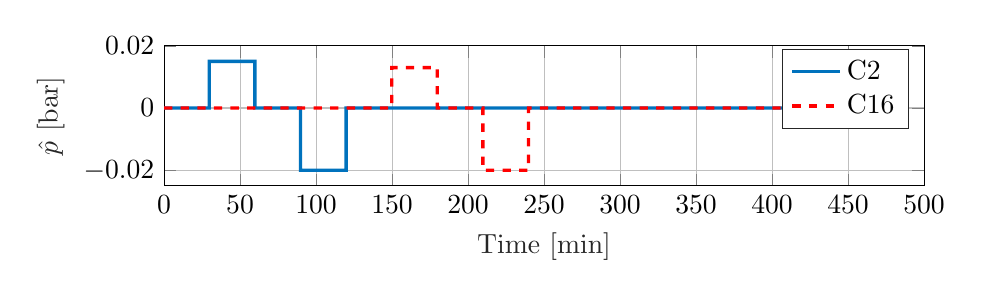
\begin{tikzpicture}

\begin{axis}[%
scaled y ticks = false,
 y tick label style={/pgf/number format/fixed,
/pgf/number format/1000 sep = \thinspace}, % Optional if you want to replace comma as the 1000 separator 
width=3.8in,
height=0.7in,
at={(1.011in,0.642in)},
scale only axis,
xmin=0,
xmax=500,
xlabel style={font=\color{white!15!black}},
xlabel={Time [min]},
ymin=-0.025,
ymax=0.02,
ylabel style={font=\color{white!15!black}},
ylabel={$\hat{p}$ [bar]},
axis background/.style={fill=white},
xmajorgrids,
ymajorgrids,
legend style={legend cell align=left, align=left, draw=white!15!black}
]
\addplot [color=mycolor1,very thick]
  table[row sep=crcr]{%
0	-0\\
29.7508333333333	-0\\
29.7516666666667	0.0149999999999864\\
59.7508333333333	0.0149999999999864\\
59.7516666666667	-0\\
89.7508333333333	-0\\
89.7516666666667	-0.0200000000000387\\
119.750833333333	-0.0200000000000387\\
119.751666666667	-0\\
478.333333333333	-0\\
};
\addlegendentry{C2}

\addplot [color=red,very thick, dashed]
  table[row sep=crcr]{%
0	-0\\
149.750833333333	-0\\
149.751666666667	0.0129999999999768\\
179.750833333333	0.0129999999999768\\
179.751666666667	-0\\
209.750833333333	-0\\
209.751666666667	-0.0200000000000387\\
239.750833333333	-0.0200000000000387\\
239.751666666667	-0\\
478.333333333333	-0\\
};
\addlegendentry{C16}

\end{axis}
\end{tikzpicture}%
\end{figure}

\end{frame}

\begin{frame}{Implementation method}{Simulink}
\begin{itemize}
\item<1-> MPC control strategy for 24 hours
\item<1-> At each hour:
	 	\begin{itemize}
	 	\item<1-> Iterate $\hat{\pmb{d}}[k]$ and $c_p [k]$
	 	\item<1-> Measurement on the states 
	 	\item<1-> Apply control input $\pmb{\hat{u}_{Hp}}(1,1)$
	 	\end{itemize}
\end{itemize}

\begin{figure}[H]
\centering
\begin{tikzpicture} [scale=0.67,transform shape]

\draw  (10,2) rectangle (6,0);
\node at (8,1) {Model};
\node at (9.7,1.7) {$\hat{y}$};
\node at (9.7, 0.3) {$\hat{x}$};
\node at (6.3, 1.7) {$\hat{d}$};
\node at (6.3, 0.3) {$\hat{u}$};
\draw[-triangle 60] (10, 1.7) -- (11, 1.7);

\draw[-triangle 60] (10, 0.3) -- (11, 0.3) -- (11,-3) -- (9,-3);

\draw  (9,-2) rectangle (7,-4);
\node at (8,-3) {MPC};
\node at (6.5,-2.55) {$\pmb{\hat{u}_{Hp}}$};
\draw  (7,-3) -- (6,-3);
\draw (6,-3.3) rectangle (4,-2.7);
\draw (8.5,2) rectangle (7.9,1.5);
\node at (8.2,1.8) {$T_s$};

\draw  (5.8,-3.3) -- (5.8,-2.7);
\draw  (5.6,-3.3) -- (5.6,-2.7);
\draw  (5.4,-3.3) -- (5.4,-2.7);
\draw  (5.2,-3.3) -- (5.2,-2.7);
\draw  (5.0,-3.3) -- (5.0,-2.7);
\draw  (4.8,-3.3) -- (4.8,-2.7);
\draw  (4.6,-3.3) -- (4.6,-2.7);
\draw  (4.4,-3.3) -- (4.4,-2.7);
\draw  (4.2,-3.3) -- (4.2,-2.7);
\fill[ForestGreen] (4.18,-3.29) rectangle(4.01,-2.71);
\draw[-triangle 60] (4, -3) -- (3, -3) -- (3,0.3) -- (6,0.3);
\node at (3.9,-1.5) {$\pmb{\hat{u}_{Hp}}(1,1)$};
\draw[-triangle 60] (5,1.7)--(6,1.7);

 
    \draw (0,1.7) -- (4.3,1.7);
    \node [font=\large] at (4.3,1.5) {t};
    \draw (0,2.4)node[left,font=\large] {$\hat{OD}$} -- (0,1.0);
    % \draw (0.2,-1)node[left,font=\tiny] {$y=-1$} -- (11.8,-1); 
    % \foreach \x in {0,0.5,...,12}{
    % \draw (\x,-0.2)node [below,font=\tiny,] {\x} -- (\x,0.2) ;
    % }
    \draw[ thick, red] (0,1.7) sin (0.7,2.4);    %% the real business in this line
    \draw[ thick, red] (0.7,2.4) cos (1.4,1.7);    %% the real business in this line
    \draw[ thick, red] (1.4,1.7) sin (2.1,0.9);    %% the real business in this line
    \draw[ thick, red] (2.1,0.9) cos (2.8,1.7);    %% the real business in this line
    \draw[ thick, red] (2.8,1.7)  sin (3.5,2.4);    %% the real business in this line
    \draw[ thick, red] (3.5,2.4) cos (4.2,1.7);    %% the real business in this line
    % \draw[ultra thick, red] (9,0) sin (10,-1);    %% the real business in this line
    % \draw[ultra thick, blue] (10,-1) cos (11,0);    %% the real business in this line

\end{tikzpicture}%


 
\end{figure}

\end{frame}


\subsection{Implementation results}

\begin{frame}{Implementation results}{For one iteration}

\begin{itemize}
	 	\item<1-> Softened constraints on $\hat{\pmb{\underline{u}}}_{Hp}$
	 	\end{itemize}

\begin{figure}[H]
   \centering
    % This file was created by matlab2tikz.
%
%The latest updates can be retrieved from
%  http://www.mathworks.com/matlabcentral/fileexchange/22022-matlab2tikz-matlab2tikz
%where you can also make suggestions and rate matlab2tikz.
%
\definecolor{mycolor1}{rgb}{0.00000,0.44700,0.74100}%
%
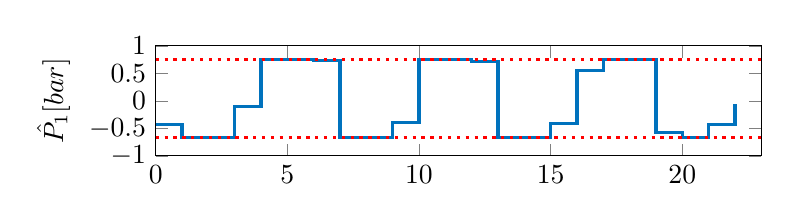
\begin{tikzpicture}

\begin{axis}[%
width=3.028in,
height=0.55in,at={(1.011in,4.137in)},
scale only axis,
xmin=0,
xmax=23,
ymin=-1,
ymax=1,
ylabel={$\hat{P_1}[bar]$},
%xmajorgrids,
%ymajorgrids,
axis background/.style={fill=white},
title style={font=\bfseries},
%title={$\text{u}_{\text{hp1}}\text{[k=0]}$}
]
\addplot[const plot,color=mycolor1,solid,forget plot,very thick] plot table[row sep=crcr] {%
0	-0.433446931217239\\
1	-0.669999999998947\\
2	-0.669999999997713\\
3	-0.104236955958482\\
4	0.749999999997401\\
5	0.749999999998619\\
6	0.727077455814283\\
7	-0.669999999999055\\
8	-0.66999999999925\\
9	-0.395725243988171\\
10	0.749999999988271\\
11	0.749999999998319\\
12	0.717572940373614\\
13	-0.669999999998221\\
14	-0.669999999999149\\
15	-0.409583761852645\\
16	0.548034702463677\\
17	0.749999999998184\\
18	0.74999999999883\\
19	-0.576396407197271\\
20	-0.669999999998877\\
21	-0.425048538821507\\
22	-0.0640667111129486\\
};
\addplot[const plot,color=red,dotted,very thick] plot table[row sep=crcr] {%
0	0.75\\
24	0.75\\
};

\addplot[const plot,color=red,dotted,very thick] plot table[row sep=crcr] {%
0	-0.67\\
24	-0.67\\
};

\end{axis}
\end{tikzpicture}


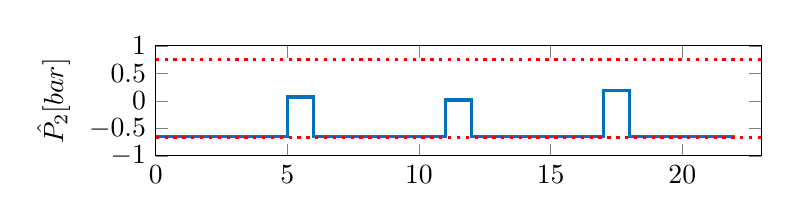
\begin{tikzpicture}

\begin{axis}[%
width=3.028in,
height=0.55in,
at={(1.011in,2.39in)},
scale only axis,
xmin=0,
xmax=23,
ymin=-1,
ymax=1,
%xmajorgrids,
%ymajorgrids,
ylabel={$\hat{P_2}[bar]$},
axis background/.style={fill=white},
title style={font=\bfseries},
%title={$\text{u}_{\text{hp2}}\text{[k=0]}$}
]
\addplot[const plot,color=mycolor1,solid,forget plot,very thick] plot table[row sep=crcr] {%
0	-0.649999999999008\\
1	-0.649999999999539\\
2	-0.649999999999527\\
3	-0.64999999999887\\
4	-0.649999999994262\\
5	0.0667700518106753\\
6	-0.649999999998485\\
7	-0.649999999999511\\
8	-0.649999999999588\\
9	-0.649999999999157\\
10	-0.649999999997306\\
11	0.0160826405819198\\
12	-0.649999999996155\\
13	-0.64999999999941\\
14	-0.64999999999958\\
15	-0.649999999999219\\
16	-0.649999999998156\\
17	0.189015571020597\\
18	-0.649999999956971\\
19	-0.649999999999335\\
20	-0.649999999999555\\
21	-0.649999999999218\\
22	-0.649999999998207\\
};
\addplot[const plot,color=red,dotted,very thick] plot table[row sep=crcr] {%
0	0.75\\
24	0.75\\
};

\addplot[const plot,color=red,dotted,very thick] plot table[row sep=crcr] {%
0	-0.67\\
24	-0.67\\
};
\end{axis}
\end{tikzpicture}

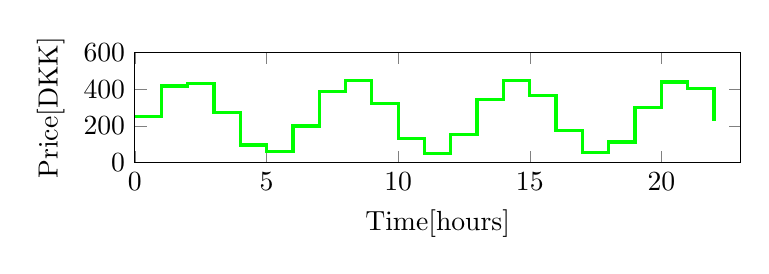
\begin{tikzpicture}

\begin{axis}[%
width=3.028in,
height=0.55in,
at={(1.011in,0.642in)},
scale only axis,
xmin=0,
xmax=23,
xlabel={Time[hours]},
ymin=0,
ymax=600,
%xmajorgrids,
%ymajorgrids,
ylabel={Price[DKK]},
axis background/.style={fill=white},
title style={font=\bfseries},
]
\addplot[const plot,color=green,solid,forget plot,very thick] plot table[row sep=crcr] {%
0	250\\
1	418.857649358291\\
2	430.978019589665\\
3	275.110723996831\\
4	95.9351176989303\\
5	59.7658279797972\\
6	200.175962602534\\
7	386.833833626164\\
8	446.479615730073\\
9	323.748819156816\\
10	132.562792409559\\
11	50.3844917318038\\
12	153.493572208496\\
13	346.181981592006\\
14	449.592219965457\\
15	367.736693884804\\
16	176.595452155304\\
17	53.5898806097876\\
18	112.896379753435\\
19	299.465389524004\\
20	440.119567515206\\
21	404.300699515516\\
22	225.256624358491\\
};
\end{axis}
\end{tikzpicture}%
\end{figure}

\end{frame}


\section{Discussion}
\begin{frame}{Discussion}{}

\begin{itemize}
	\item<1->Linear/nonlinear model comparison
	\begin{itemize}
	 \item<1-> Online linearization
	 \item<1-> Operating points are constantly varied
	 \item<1-> Precision is more reliable

	\end{itemize}
\end{itemize}

\begin{itemize}
\item<2-> Considerations for the future
	 \begin{itemize}
	 \item<2-> Long measurements, ensuring initial steady state condition
	 \item<2-> Softening constraints
	 \item<2-> Using the end-user pressure measurements
	 \item<2-> Robust MPC
	 \end{itemize}
\end{itemize}

\end{frame}
